% Created 2013-05-07 Ter 00:37
\documentclass[a4paper]{article}
\usepackage{times}
\usepackage[utf8]{inputenc}
\usepackage[T1]{fontenc}
\usepackage{graphicx}
%\usepackage{amssymb}
\usepackage{hyperref}
\linespread{1.5}	% double spaces lines
\usepackage[hmargin=3cm,vmargin=3cm]{geometry}
\usepackage{indentfirst}
\usepackage{amsmath}
\usepackage{amsthm}
\usepackage{sectsty}
\usepackage{enumitem}
\usepackage[brazil]{babel}
\usepackage{placeins} %mantem figuras na secao com \FloatBarrier
\usepackage{txfonts}
\usepackage{textcomp} % \textcurrency
\hypersetup{%
    pdfborder = {0 0 0}
}




\begin{document}

\begin{center}


\uppercase{\large Universidade Federal do Rio Grande do Sul\\

\large Instituto de Informática \\

\large Curso de Ciência da Computação \\

\large Teoria da Computação N (2014/1)\\
}

\large Prof. Dr. Tiarajú Asmuz Diverio \\

\large Graduandos: \\ Paulo Renato Lanzarin, Ricardo Gabriel Herdt (Turma C) e \\
	Wladimir Leuschner (Turma B) \\[1cm]

% Title
\large \bfseries Máquinas fatorial e ordena \\[1.0cm]



% Bottom of the page

\end{center}


\section{Fatorial}
A máquina $\mathbf{fatorial}$ é definida como:
\begin{equation*}
\mathbf{fatorial} = (\{1\}, \{q_0, q_1, ..., q_{19}, q_{20}\}, T, q_0,
\{q_3, q_{22}, q_{24}\}, \{A, B, C, D\}, \beta, \text{\textcurrency} )\end{equation*} onde $\mathbf{T}$ é a função de transição descrita na tabela 1.

A máquina $\mathbf{fatorial}$ recebe um valor numérico $n$ e computa $n!$. Os 
números são representados em unário sobre o alfabeto \{1\}. \\[1.0cm]

\begin{table}[h!]
  \centering
  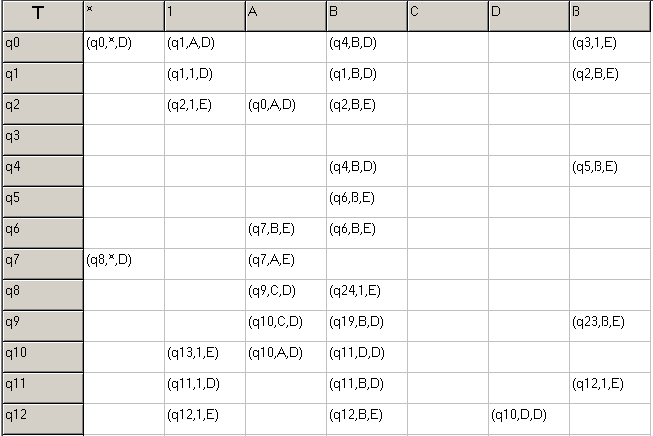
\includegraphics[scale=0.5]{fatorial_1.png}
\end{table}

\begin{table}[t!]
  \centering
  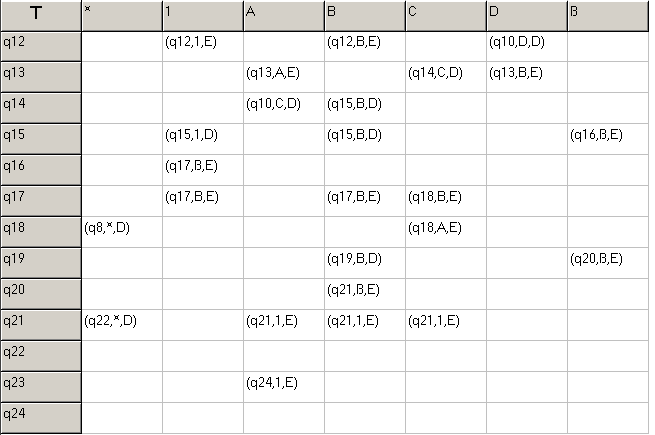
\includegraphics[scale=0.5]{fatorial_2.png}
  \caption{\textbf{fatorial}}
\end{table}

\section{Ordena}

A máquina $\mathbf{ordena}$ é definida como:
\begin{equation*}
\mathbf{ordena} = (\{1\}, \{q_0, q_1, q_2, q_3, q_4, q_5, q_6, q_7, q_8, q_9, q_{10}, q_{11}\}, O, q_0,
\{q_4\}, \emptyset, \beta, \text{\textcurrency} )\end{equation*} onde $\mathbf{O}$ é a função de transição descrita na tabela 2.

Ela ordena uma palavra de entrada sobre o alfabeto \{a, b, c\}, empregando o 
algoritmo de ordenamento \emph{Bubble sort}.

\begin{table}[b!]
  \centering
  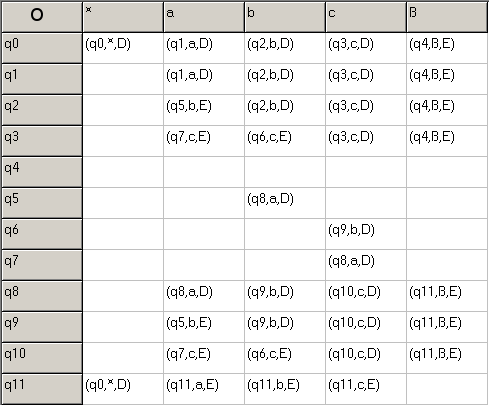
\includegraphics[scale=0.5]{ordena.png}
  \caption{\textbf{ordena}}
\end{table}

\end{document}
